\documentclass[14pt]{extbook}
\usepackage{multicol, enumerate, enumitem, hyperref, color, soul, setspace, parskip, fancyhdr} %General Packages
\usepackage{amssymb, amsthm, amsmath, latexsym, units, mathtools} %Math Packages
\everymath{\displaystyle} %All math in Display Style
% Packages with additional options
\usepackage[headsep=0.5cm,headheight=12pt, left=1 in,right= 1 in,top= 1 in,bottom= 1 in]{geometry}
\usepackage[usenames,dvipsnames]{xcolor}
\usepackage{dashrule}  % Package to use the command below to create lines between items
\newcommand{\litem}[1]{\item#1\hspace*{-1cm}\rule{\textwidth}{0.4pt}}
\pagestyle{fancy}
\lhead{Progress Quiz 8}
\chead{}
\rhead{Version A}
\lfoot{5493-4176}
\cfoot{}
\rfoot{Summer C 2021}
\begin{document}

\begin{enumerate}
\litem{
Solve the modeling problem below, if possible.
\begin{center}
    \textit{ A new virus is spreading throughout the world. There were initially 6 many cases reported, but the number of confirmed cases has quadrupled every 4 days. How long will it be until there are at least 1000 confirmed cases? }
\end{center}
\begin{enumerate}[label=\Alph*.]
\item \( \text{About } 9 \text{ days} \)
\item \( \text{About } 21 \text{ days} \)
\item \( \text{About } 15 \text{ days} \)
\item \( \text{About } 10 \text{ days} \)
\item \( \text{There is not enough information to solve the problem.} \)

\end{enumerate} }
\litem{
Solve the modeling problem below, if possible.
\begin{center}
    \textit{ A new virus is spreading throughout the world. There were initially 5 many cases reported, but the number of confirmed cases has doubled every 4 days. How long will it be until there are at least 10000 confirmed cases? }
\end{center}
\begin{enumerate}[label=\Alph*.]
\item \( \text{About } 15 \text{ days} \)
\item \( \text{About } 44 \text{ days} \)
\item \( \text{About } 31 \text{ days} \)
\item \( \text{About } 16 \text{ days} \)
\item \( \text{There is not enough information to solve the problem.} \)

\end{enumerate} }
\litem{
For the scenario below, use the model for the volume of a cylinder as $V = \pi r^2 h$.
\begin{center}
    \textit{ Pringles wants to add 26 \text{percent} more chips to their cylinder cans and minimize the design change of their cans. They've decided that the best way to minimize the design change is to increase the radius and height by the same percentage. What should this increase be? }
\end{center}
\begin{enumerate}[label=\Alph*.]
\item \( \text{About } 8 \text{ percent} \)
\item \( \text{About } 3 \text{ percent} \)
\item \( \text{About } 13 \text{ percent} \)
\item \( \text{About } 12 \text{ percent} \)
\item \( \text{None of the above} \)

\end{enumerate} }
\litem{
For the scenario below, model the rate of vibration (cm/s) of the string in terms of the length of the string. Then determine the variation constant $k$ of the model (if possible). The constant should be in terms of cm and s.
\begin{center}
    \textit{ The rate of vibration of a string under constant tension varies based on the type of string and the length of the string. The rate of vibration of string $\omega$ decreases as the cube length of the string increases. For example, when string $\omega$ is 2 mm long, the rate of vibration is 29 cm/s. }
\end{center}
\begin{enumerate}[label=\Alph*.]
\item \( k = 0.23 \)
\item \( k = 3.62 \)
\item \( k = 3625.00 \)
\item \( k = 232.00 \)
\item \( \text{None of the above.} \)

\end{enumerate} }
\litem{
Solve the modeling problem below, if possible.
\begin{center}
    \textit{ In CHM2045L, Brittany created a 24 liter 20 percent solution of chemical $\chi$ using two different solution percentages of chemical $\chi$. When she went to write her lab report, she realized she forgot to write the amount of each solution she used! If she remembers she used 18 percent and 33 percent solutions, what was the amount she used of the 33 percent solution? }
\end{center}
\begin{enumerate}[label=\Alph*.]
\item \( 3.20 liters \)
\item \( 12.34 liters \)
\item \( 20.80 liters \)
\item \( 12.00 liters \)
\item \( \text{There is not enough information to solve the problem.} \)

\end{enumerate} }
\litem{
Determine the appropriate model for the graph of points below.
\begin{center}
    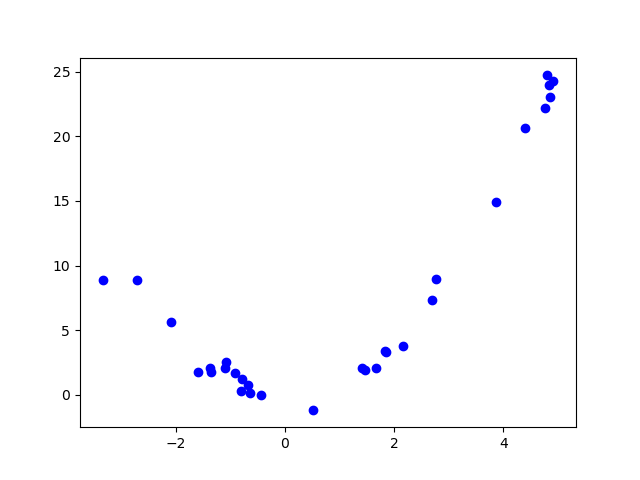
\includegraphics[width=0.5\textwidth]{../Figures/identifyModelGraph12A.png}
\end{center}
\begin{enumerate}[label=\Alph*.]
\item \( \text{Exponential model} \)
\item \( \text{Linear model} \)
\item \( \text{Non-linear Power model} \)
\item \( \text{Logarithmic model} \)
\item \( \text{None of the above} \)

\end{enumerate} }
\litem{
For the scenario below, use the model for the volume of a cylinder as $V = \pi r^2 h$ to find the coefficient for the model of the new volume $V_{\text{new}} = k r^2 h$.
\begin{center}
    \textit{ Pepsi wants to increase the volume of soda in their cans. They've decided to increase the radius by 12 percent and increase the height by 15 percent. They want to model the new volume based on the radius and height of the original cans. }
\end{center}
\begin{enumerate}[label=\Alph*.]
\item \( k = 0.00216 \)
\item \( k = 4.53194 \)
\item \( k = 1.44256 \)
\item \( k = 0.00679 \)
\item \( \text{None of the above.} \)

\end{enumerate} }
\litem{
For the scenario below, use the model for the volume of a cylinder as $V = \pi r^2 h$.
\begin{center}
    \textit{ Pringles wants to add 48 \text{percent} more chips to their cylinder cans and minimize the design change of their cans. They've decided that the best way to minimize the design change is to increase the radius and height by the same percentage. What should this increase be? }
\end{center}
\begin{enumerate}[label=\Alph*.]
\item \( \text{About } 22 \text{ percent} \)
\item \( \text{About } 4 \text{ percent} \)
\item \( \text{About } 24 \text{ percent} \)
\item \( \text{About } 14 \text{ percent} \)
\item \( \text{None of the above} \)

\end{enumerate} }
\litem{
Solve the modeling problem below, if possible.
\begin{center}
    \textit{ In CHM2045L, Brittany created a 19 liter 35 percent solution of chemical $\chi$ using two different solution percentages of chemical $\chi$. When she went to write her lab report, she realized she forgot to write the amount of each solution she used! If she remembers she used 20 percent and 42 percent solutions, what was the amount she used of the 20 percent solution? }
\end{center}
\begin{enumerate}[label=\Alph*.]
\item \( 11.11 liters \)
\item \( 9.50 liters \)
\item \( 12.95 liters \)
\item \( 6.05 liters \)
\item \( \text{There is not enough information to solve the problem.} \)

\end{enumerate} }
\litem{
Determine the appropriate model for the graph of points below.
\begin{center}
    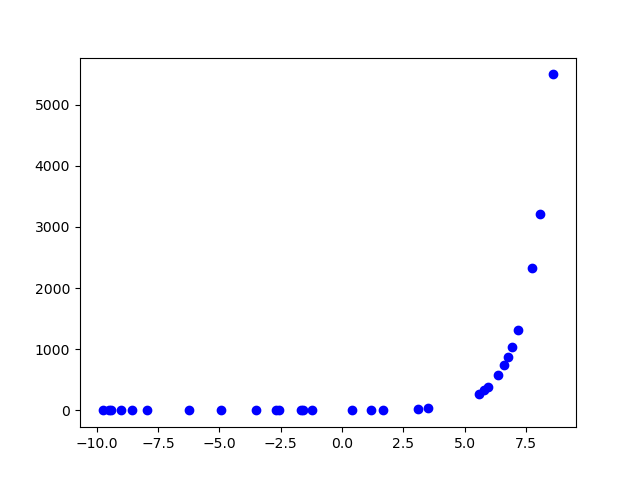
\includegraphics[width=0.5\textwidth]{../Figures/identifyModelGraph12CopyA.png}
\end{center}
\begin{enumerate}[label=\Alph*.]
\item \( \text{Non-linear Power model} \)
\item \( \text{Linear model} \)
\item \( \text{Logarithmic model} \)
\item \( \text{Exponential model} \)
\item \( \text{None of the above} \)

\end{enumerate} }
\end{enumerate}

\end{document}